%%% Exemplo de utilização da classe ITA
%%%
%%%   por        Fábio Fagundes Silveira   -  ffs [at] ita [dot] br
%%%              Benedito C. O. Maciel     -  bcmaciel [at] ita [dot] br
%%%              Giovani Volnei Meinertz   -  giovani [at] ita [dot] br
%%%    	         Hudson Alberto Bode       -  bode [at] ita [dot]br
%%%    	         P. I. Braga de Queiroz    -  pi [at] ita [dot] br
%%%    	         Jorge A. B. Gripp         -  gripp [at] ita [dot] br
%%%    	         Juliano Monte-Mor         -  jamontemor [at] yahoo [dot] com [dot] br
%%%    	         Tarcisio A. B. Gripp      -  tarcisio.gripp [at] gmail [dot] com
%%%    	         
%%%
%%%  IMPORTANTE: O texto contido neste exemplo nao significa absolutamente nada.  :-)
%%%              O intuito aqui eh demonstrar os comandos criados na classe e suas
%%%              respectivas utilizacoes.
%%%
%%%  Tese.tex  2015-04-08
%%%  $HeadURL: http://www.apgita.org.br/apgita/teses-e-latex.php $
%%%
%%% ITALUS
%%% Instituto Tecnológico de Aeronáutica --- ITA, Sao Jose dos Campos, Brasil
%%%                   http://groups.yahoo.com/group/italus/
%%% Discussion list: italus {at} yahoogroups.com
%%%
%++++++++++++++++++++++++++++++++++++++++++++++++++++++++++++++++++++++++++++++
% Parametros da classe ITA para inserir em \documentclass[?]{?}
%   tg       = Trabalho de Graduacao
%   tgfem    = Para Engenheiras
%   msc      = Dissertacao de Mestrado
%   mscfem   = Para Mestras
%   dsc      = Tese de Doutorado
%   dscfem   = Para Doutoras
%   quali    = Exame de Qualificacao
%   qualifem = Exame de Qualificacao para Doutoras
%   dv       = 'Draft Version'     --> imprime 'Versao Preliminar + data no rodape
%   eng      = para teses em inglês
%++++++++++++++++++++++++++++++++++++++++++++++++++++++++++++++++++++++++++++++
%se fosse em inglês: \documentclass[dsc, eng]{ita}
%para ``draft version'': \documentclass[dsc, dv]{ita} ou \documentclass[dsc, eng, dv]{ita}

\documentclass[tg]{ita}    % ITA.cls based on standard book.cls 
% Quando alterar a classe, por exemplo de [msc] para [msc, eng]) rode mais uma vez o botão BUILD OUTPUT caso haja erro
\usepackage{ae}
\usepackage{graphicx}
\usepackage{epsfig}
\usepackage{amsmath}
\usepackage{amssymb} 
\usepackage{subfig}
\usepackage{multirow}
\usepackage{float}

%++++++++++++++++++++++++++++++++++++++++++++++++++++++++++++++++++++++++++++++
% Espaçamento padrão de todo o documento
%++++++++++++++++++++++++++++++++++++++++++++++++++++++++++++++++++++++++++++++
\onehalfspacing

%singlespacing Para um espaçamento simples
%onehalfspacing Para um espaçamento de 1,5
%doublespacing Para um espaçamento duplo

%++++++++++++++++++++++++++++++++++++++++++++++++++++++++++++++++++++++++++++++
% Identificacoes (se o trabalho for em inglês, insira os dados em inglês)
% Para entradas abreviadas de Professora (Profa.) em português escreva: Prof$^\textnormal{a}$.
%++++++++++++++++++++++++++++++++++++++++++++++++++++++++++++++++++++++++++++++
\course{Engenharia de Computação} % Programa de PG ou Curso de Graduação
\dept{Engenharia de Computação} % Divisão Acadêmica no ITA

% Autor do trabalho: Nome Sobrenome
\authorgender{masc}                     %sexo: masc ou fem
\author{Gustavo Ceci}{Guimarães}
\itaauthoraddress{Rua H8B 238}{12.228-461}{São José dos Campos--SP}

% Titulo da Tese/Dissertação
\title{Desenvolvimento de uma framework em C++ para criação de jogos 3d para a Web - TG1}

% Orientador
\advisorgender{masc}                    % masc ou fem
\advisor{Prof.~Dr.}{Edgar Toshihiro Yano}{ITA}

%Coordenador do curso no caso de TG
\bosscoursegender{fem}									% masc ou fem
\bosscourse{Prof.~Dr.}{Cecilia César}

% Palavras-Chaves informadas pela Biblioteca -> utilizada na CIP
\kwcip{Jogos}
\kwcip{WebGL}
\kwcip{OpenGL}
\kwcip{WebAssembly}
\kwcip{Emscripten}
\kwcip{C++}

% TODO: membros da banca examinadora

\examiner{Prof. Dr.}{Alan Turing}{Presidente}{ITA}
\examiner{Prof. Dr.}{Linus Torwald}{}{UXXX}
\examiner{Prof. Dr.}{Richard Stallman}{}{UYYY}
\examiner{Prof. Dr.}{Donald Duck}{}{DYSNEY}
\examiner{Prof. Dr.}{Mickey Mouse}{}{DISNEY}

% TODO: Data da defesa (mês em maiúsculo, se trabalho em inglês, e minúsculo se trabalho em português) 
\date{5}{março}{2015}

% TODO: Número CDU - (somente para TG)
\cdu{621.38}

% Glossario
\makeglossary
\frontmatter

\begin{document}
% Folha de Rosto e Capa para o caso do TG
\maketitle

% Dedicatoria: Nao esqueca essa secao  ... :-)
\begin{itadedication}
Aos meus queridos amigos
\end{itadedication}

% Agradecimentos
\begin{itathanks}
Primeiramente, gostaria de agradecer ao Dr. Donald E. Knuth, por ter desenvolvido o \TeX.

Ao Dr. Leslie Lamport, por ter criado o \LaTeX, facilitando muito a utilização do \TeX, e assim, eu não ter que usar o Word.

Ao Prof. Dr. Meu Orientador, pela orientação e confiança depositada na realização deste trabalho.

Ao Dr. Nelson D'Ávilla, por emprestar seu nome a essa importante via de trânsito na cidade de São José dos Campos.

Ah, já estava esquecendo... agradeço também, mais uma vez ao \TeX, por ele não possuir vírus de macro :-)

\end{itathanks}

% Epígrafe
\thispagestyle{empty}
\ifhyperref\pdfbookmark[0]{\nameepigraphe}{epigrafe}\fi
\begin{flushright}
\begin{spacing}{1}
\mbox{}\vfill
{\sffamily\itshape
Não tem como dar errado.
}
\end{spacing}
\end{flushright}

% Resumo
\begin{abstract}
Aqui começa o resumo do referido trabalho. Não tenho a menor idéia do que colocar aqui. Sendo assim, vou inventar. Lá vai: Este trabalho apresenta uma metodologia de controle de posição das juntas passivas de um manipulador subatuado de uma maneira subótima. O termo subatuado se refere ao fato de que nem todas as juntas ou graus de liberdade do sistema são equipados com atuadores, o que ocorre na prática devido a falhas ou como resultado de projeto. As juntas passivas de manipuladores desse tipo são indiretamente controladas pelo movimento das juntas ativas usando as características de acoplamento da dinâmica de manipuladores. A utilização de redundância de atuação das juntas ativas permite a minimização de alguns critérios, como consumo de energia, por exemplo.
Apesar da estrutura cinemática de manipuladores subatuados ser idêntica a do totalmente atuado, em geral suas caraterísticas dinâmicas diferem devido a presença de juntas passivas. Assim, apresentamos a modelagem dinâmica de um manipulador subatuado e o conceito de índice de acoplamento. Este índice é utilizado na sequência de controle ótimo do \mbox{manipulador}.
A hipótese de que o número de juntas ativas seja maior que o número de
passivas  $(n_{a} > n_{p})$  permite o controle ótimo das juntas passivas, uma vez que na etapa
de controle destas há mais entradas (torques nos atuadores das juntas ativas), que
elementos a controlar (posição das juntas passivas). 
\end{abstract}

% Abstract
\begin{englishabstract}

Well, the book is on the table. This work presents a control methodologie for the position of the  passive joints of an underactuated manipulator in a suboptimal way. The term underactuated refers to the fact that not all the joints or degrees of freedom of the system are equipped with actuators, which occurs in practice due to failures or as design result. The passive joints of manipulators like this are indirectly controlled by the motion of the active joints using the dynamic coupling characteristics. The utilization of actuation redundancy of the active joints allows the minimization of some criteria, like energy consumption, for example. Although the kinematic structure of an underactuated manipulator is identical to that of a similar fully actuated one, in general their dynamic characteristics are different due to the presence of passive joints. Thus, we present the dynamic modelling of an underactuated manipulator and the concept of coulpling index. This index is used in the sequence of the optimal control of the manipulator.

\end{englishabstract}

% Lista de figuras
\listoffigures %opcional

% Lista de tabelas
\listoftables %opcional

% Lista de abreviaturas
\listofabbreviations
\begin{longtable}{ll}
CTq & computed torque \\
DC & direct current \\
EAR & Equação Algébrica de Riccati \\
GDL & graus de liberdade \\
ISR & interrupção de serviço e rotina \\
LMI & linear matrices inequalities \\
MIMO & multiple input multiple output \\
PD & proporcional derivativo \\
PID & proporcional integrativo derivativo \\
PTP & point to point \\
UARMII & Underactuated Robot Manipulator II \\
VSC & variable structure control \\

\end{longtable}

 %opcional

% Lista de simbolos
\listofsymbols
\begin{longtable}{ll}
$a$ & Distância\\
$\textbf{a}$ & Vetor de distâncias\\
$\textbf{e}_{j}$ & Vetor unitário de dimensão $n$ e com o $j$-ésimo componente igual a $1$ \\
$\textbf{K}$ & Matriz de rigidez\\
$m_1$ & Massa do cumpim\\
$\delta_{k-k_f}$ & Delta de Kronecker no instante $k_f$\\

\end{longtable}

 %opcional

% Sumario
\tableofcontents

\mainmatter
% Os capitulos comecam aqui

\chapter{Introdução}

A indústria de jogos é um dos setores da indústria de entretenimento que mais gera lucro, gerando em 2016 mais lucro que o setor de musica e de filmes \cite{NASDAQ}. Essa indústria é dividida em diversos outros subsetores como o desenvolvimento de jogos para video-game, jogos mobile e jogos de computador. Dentro do setor dos jogos de computador pode-se tambem fazer algumas subdivisões como jogos que precisam ser instalados e jogos que podem ser jogados no browser.

Apesar de ser a menor parcela do setor no quesito de lucro, os jogos de browser ainda possuem relevância no contexto geral, e muitas vezes servem como o ambiente inicial onde o jogo pode ser jogado \cite{NEWZOO}. Por não necessitarem de software baixado além do navegador e serem tipicamente gratuitos, os jogos de browser são de acessibilidade muito simples para o usuário. Para os desenvolvedores, especialmente aqueles sem investimentos multimilionários voltados para marketing e publicação, a acessibilidade dos jogos de browser torna-se um método de veículação e engajamento de usuário muito eficiente. Diversos jogos independentes bem sucedidos possuem ou possuiram em algum momento alguma versão ou protótipo possivel de ser jogado no browser \cite{BOI, CLICKERHEROES, SUPERHOT}.

Além do apelo financeiro, jogos podem ser usados como forma de expressão artística e como um hobby. Como para as grandes empresas jogos são um investimento multimilionário, os resultados são em sua maioria jogos menos inovadores que aqueles desenvolvidos por pequenas empresas ou desenvolvedores que o fazem por hobby, uma vez que o risco envolvido para estes costuma ser bem menor \cite{CREATINGGAMES}.

Inicialmente, grande parte dos jogos de browser eram desenvolvidos utilizando-se a ferramenta Adobe Flash, porém, com o surgimento do HTML5 e do WebGL, o uso de um plugin terceirizado para rodar jogos tem sido cada vez mais mal visto, incentivando o desenvolvimento usando as tecnologias padrão encontradas no browser \cite{UNITYWEB, FLASH}.

Uma limitação sempre presente quanto à evolução dos jogos de browser é a limitação da velocidade de processamento do browser, especialmente quando os jogos são em ambientes tridimensionais. A linguagem mais utilizada para o desenvolvimento de jogos 3d é C++, especialmente devido à eficiência, gerenciamento de memória e comunicação com sistemas de baixo nível como a placa de video. Como javascript é a linguagem padrão dos browsers e sua eficiência é consideravelmente inferior à de C++ \cite{BENCHMARK}, a implementação de jogos 3d com graficos otimizados no browser sempre foi deixada de lado. No entanto com o crescimento cada vez maior das tecnologias dos browsers tornou-se necessário cada vez mais ter códigos mais eficientes e com velocidades mais próximas à nativa, surgindo assim diversas soluções para se executar codigos nativos no browser como PNaCL \cite{PNACL} e WebAssembly \cite{WASM}.

\section{Motivação}

As ferramentas existentes hoje em dia para desenvolvimento de jogos com suporte para exportar para web são em sua maioria Engines completas, como Unity3d, Unreal Engine e Godot. Estas possuem inúmeras utilidades como simulação de física, criação de interface de usuário (UI), gerenciador de animações para modelos 3d, entre outras. Para ser possível a união de tantas ferramentas em uma unica Engine, o usuário acaba se vinculando demais à arquitetura da mesma e soluções improváveis acabam se tornando mais difíceis de se implementar devido à generalização. Para a maioria dos casos a Engine serve perfeitamente ao desenvolvedor, no entanto, em alguns casos a falta de controle é relevante.

Esse trabalho tem como objetivo criar não uma engine, mas uma framework que dá ao usuário a capacidade de pular as tarefas mais complicadas de se desenvolver uma engine, como um mecanismo simples de input e uma interface mais simples de utilização da placa de vídeo que o OpenGL padrão.

A motivação pessoal para o desenvolvimento desse trabalho é poder ter uma ferramenta propria para desenvolvimento de jogos, com capacidade de exportar para Web. Além disso, esse projeto visa ampliar os conhecimentos sobre os sistemas de baixo nível no desenvolvimento de jogos, especialmente um melhor entendimento de API's de gráfico 3d e da linguagem C++ em um projeto de maior escala.

\section{Objetivo}

O objetivo do trabalho é ter uma framework de facil distribuição e fácil uso no sistema operacional Windows. Para a criação de jogos, a framework terá como objetivo abstrair as camadas de entendimento complexo relacionado ao uso do OpenGL e do STL. A framework deverá ter uma interface simples de posicionamento de formas geométricas no espaço (sendo um bonus a possibilidade de se importar modelos 3d) além da implementação de um sistema de cameras básico. Além disso, a framework deverá possuir uma interface simples de leitura de input do teclado e do mouse. Por fim, caso se mostre necessário, a framework poderá ter integrada uma biblioteca de UI imediata para casos de debug e desenvolvimento.

\section{Ferramentas}
%Sequencia de passos necessários para demonstrar que o objetivo proposto foi atingido, ou seja, que os resultados obtidos são convincentes
\subsection{Emscripten}
Emscripten é um compilador de LLVM para javascript. LLVM é uma infraestrutura de compilador que serve para facilitar a criação de compiladores e transpiladores. Dada qualquer linguagem compilada para a linguagem intermediária do LLVM, a ferramenta Emscripten pode ser utilizada para ser enfim compilada pra javascript \cite{EMSCRIPTEN}.

O principal objetivo de compilar LLVM para javascript é a compilação de C++. Além disso, o Emscripten possui já implementadas algumas bibliotecas importantes para o uso no browser, sendo elas a transformação de OpenGL para WebGL e a biblioteca SDL2.

\subsection{OpenGL}
OpenGL, \textit{Open Graphics Library} é uma API multiplataforma padrão para desenvolvimento de graficos 3D. É um padrão de API 3D amplamente aceito com uso significante no mundo real.\cite{OPENGL}. A versão do OpenGL usada nos browsers, com a API em javascript é conhecida como WebGL, que é baseada no OpenGL ES 2.0, versão essa voltada para dispositivos móveis e sistemas embarcados. Como o emscripten é capaz de transformar um subconjunto de OpenGL ES 2.0 em WebGL sem maiores problemas \cite{EMSCRIPTEN_OPENGL}, esse será o subconjunto utilizado no projeto.

\subsection{SDL2}
SDL2, \textit{Simple DirectMedia Layer} é uma biblioteca de desenvolvimento multiplataforma criada para prover acesso de baixo nível aos hardwares de audio, mouse, teclado, joystick, alem de possuir uma interface com OpenGL \cite{SDL2}. Como é uma biblioteca muito utilizada para desenvolvimento de jogos em C++ e o emscripten já possui uma versão própria da biblioteca já compilada, essa foi a escolha de biblioteca base para a multimídia do trabalho.
\chapter{Modelagem Dinâmica de Cupins Cibernéticos}
\chapter{Controle Robusto de Concretos Caóticos}
\chapter{Considerações Finais}

O objetivo geral proposto foi cumprido com sucesso. Foi feita uma implementação de uma framework simples, nos moldes da framework Love2D e XNA, com simplificações. Alem disso foram implementadas algumas funcionalidades não propostas no objetivo que facilitam profundamente a implementação de um jogo, em especial o sistema de eventos e o de chamadas temporais.

O projeto pode ser continuado através da implementação de mais funcionalidades nele para expandir ainda mais o leque de possibilidades de implementação de jogos com a framework.

Algumas funcionalidades já planejadas para a framework são:

\subsection{Alta prioridade}
\begin{itemize}
  \item Permitir o uso de uma biblioteca de UI imediata para permitir alterações em parametros do jogo em tempo real e criação de uma interface de desenvolvimento durante o jogo.
  \item Implementação de um importador de modelos 3d e criação de mais algumas formas geométricas como: triangulo, quadrado, esfera e piramide.
  \item Implementar a utilização de texturas, para que seja possível que os objetos tenham não só uma unica cor, mas desenhos mais complexos.
\end{itemize}

\subsection{Media prioridade}
\begin{itemize}
  \item Fazer com que a camera possa renderizar para lugares diferentes da tela (fazer 2 camera que mostram coisas diferentes em cada metade da tela),
  \item Melhorar a performance para suportar ainda mais objetos em cena.
\end{itemize}

\subsection{Baixa prioridade}
\begin{itemize}
  \item Extensão da interface input\_handler para receber inputs de joysticks, e tambem criação de uma classe KeyboardMouseInput, que junta teclado e mouse em uma única funcionalidade.
  \item Expandindo as melhorias da camera e da textura, porém outra tarefa de igual dificuldade, seria poder colocar a imagem da camera em uma textura, abrindo margem para diversas possibilidades graficas, como espelhos.
\end{itemize}

% REFERENCIAS BIBLIOGRAFICAS
\renewcommand\bibname{\itareferencesnamebabel} %renomear título do capítulo referências
\bibliography{Referencias/referencias}

% Apendices
\appendix
\chapter{Tópicos de Dilema Linear} %opcional
\section{Uma Primeira Seção para o Apêndice}

A matriz de Dilema Linear $M$ e o vetor de torques inerciais $b$,
utilizados na simulação são calculados segundo a formulação 
abaixo:
\begin{equation}
M=\left[ \begin{array}{ccc}
M_{11} & M_{12} & M_{13} \\
M_{21} & M_{22} & M_{23} \\
M_{31} & M_{32} & M_{33}
\end{array} \right]
\end{equation}

\begin{figure}[h]
\centering
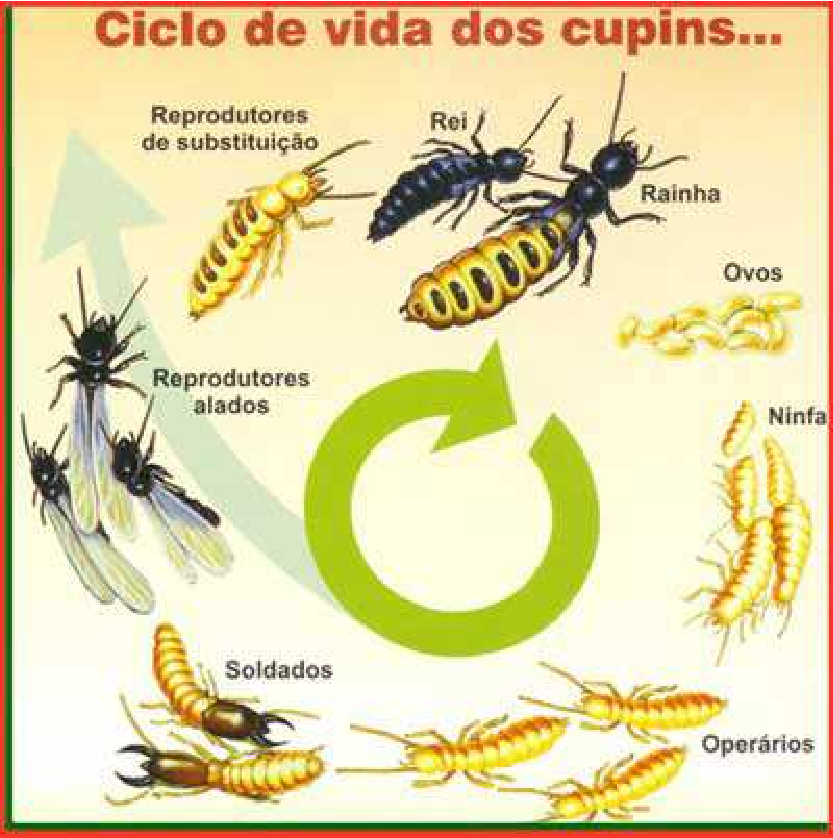
\includegraphics[height=5cm, width=5cm]{ApeA/pragas_ciclo_cupim}
\caption{Uma figura que está no apêndice}\label{FD}
\end{figure}


% Anexos
\annex
\chapter{Exemplo de um Primeiro Anexo} %opcional




% Glossario
%\itaglossary
%\printglossary

% TODO: Folha de Registro do Documento
% Valores dos campos do formulario
\FRDitadata{25 de março de 2015}
\FRDitadocnro{DCTA/ITA/TC-018/2015} %(o número de registro você solicita a biblioteca)
\FRDitaorgaointerno{Instituto Tecnológico de Aeronáutica -- Divisão de Engenharia Mecânica -- ITA/IEM}
%Exemplo no caso de pós-graduação: Instituto Tecnol{\'o}gico de Aeron{\'a}utica -- ITA
\FRDitapalavrasautor{Cupim; Cimento; Estruturas}
\FRDitapalavrasresult{Cupim; Dilema; Construção}
%Exemplo no caso de graduação (TG):
%\FRDitapalavraapresentacao{Trabalho de Graduação, ITA, São José dos Campos, 2015. \NumPenultimaPagina\ páginas.}
%Exemplo no caso de pós-graduação (msc, dsc):
\FRDitapalavraapresentacao{ITA, São José dos Campos. Curso de Mestrado. Programa de Pós-Graduação em Engenharia Aeronáutica e Mecânica. Área de Sistemas Aeroespaciais e Mecatrônica. Orientador: Prof.~Dr. Adalberto Santos Dupont. Coorientadora: Prof$^\textnormal{a}$.~Dr$^\textnormal{a}$. Doralice Serra. Defesa em 05/03/2015. Publicada em 25/03/2015.}
\FRDitaresumo{Aqui começa o resumo do referido trabalho. Não tenho a menor idéia do que colocar aqui. Sendo assim, vou inventar. Lá vai: Este trabalho apresenta uma metodologia de controle de posição das juntas passivas de um manipulador subatuado de uma maneira subótima. O termo subatuado se refere ao fato de que nem todas as juntas ou graus de liberdade do sistema são equipados com atuadores, o que ocorre na prática devido a falhas ou como resultado de projeto. As juntas passivas de manipuladores desse tipo são indiretamente controladas pelo movimento das juntas ativas usando as características de acoplamento da dinâmica de manipuladores. A utilização de redundância de atuação das juntas ativas permite a minimização de alguns critérios, como consumo de energia, por exemplo.
Apesar da estrutura cinemática de manipuladores subatuados ser idêntica a do totalmente atuado, em geral suas caraterísticas dinâmicas diferem devido a presença de juntas passivas. Assim, apresentamos a modelagem dinâmica de um manipulador subatuado e o conceito de índice de acoplamento. Este índice é utilizado na sequência de controle ótimo do \mbox{manipulador}.
A hipótese de que o número de juntas ativas seja maior que o número de
passivas  $(n_{a} > n_{p})$  permite o controle ótimo das juntas passivas, uma vez que na etapa
de controle destas há mais entradas (torques nos atuadores das juntas ativas), que
elementos a controlar (posição das juntas passivas). }
%  Primeiro Parametro: Nacional ou Internacional -- N/I
%  Segundo parametro: Ostensivo, Reservado, Confidencial ou Secreto -- O/R/C/S
\FRDitaOpcoes{N}{O}
% Cria o formulario
\itaFRD

\end{document}
% Fim do Documento. O massacre acabou!!! :-)
